% Chapter 3.4: Subsurface Multiphase Flow and Carbon Storage
% Part III of the book.

\chapter{Subsurface Multiphase Flow and Carbon Storage}
\label{ch:part3-subsurface-multiphase-flow-and-carbon-stor}
\label{sec:subsurface}
% -----------------------------------------------------------------------------

Geological carbon storage is a forecasting problem that sits on the wrong side of
every budget a numerical simulator has. Carbon capture and storage (CCS) requires
injecting $\mathrm{CO}_2$, compressed into a supercritical fluid above its critical
point at roughly $31.0\,^\circ\mathrm{C}$ and $7.38\,\mathrm{MPa}$, into deep
saline aquifers, and then predicting where the gas saturation plume will be and how
far the reservoir pressure will have risen, on injection horizons of decades and
migration horizons of centuries.
\index{carbon capture and storage (CCS)}
The mechanism that makes the practice possible is what makes the prediction hard:
supercritical $\mathrm{CO}_2$ is substantially lighter than the brine it displaces,
so it rises until a low-permeability caprock stops it.
\index{caprock!containment role}
The questions a regulator or a nearby groundwater user asks concern that caprock,
the faults, and the abandoned wellbores: how far the pressure front travels, and
whether the plume reaches a leaky pathway.

Classical solvers strain under two pressures at once. The first is the equation
system: two-phase flow in a porous medium is nonlinear, coupled, and of mixed
elliptic--hyperbolic type, and its saturation fronts are genuine discontinuities
whose speed is set by a jump condition rather than by smooth characteristics. The
second is the workflow. Permeability is measured at a handful of well cores and
interpolated statistically in between, so no single simulation is a prediction; the
decision-relevant object is a distribution over outcomes, which means solving the
same problem thousands of times on different geological realizations. That is the
multi-query pattern of
\chapref{ch:part3-the-multi-query-bottleneck-in-computationa} in its purest form.

Parts~I and~II supply the machinery and, more importantly, the doubts. Part~I
gives the spectral layer \eqref{eq:fno_layer}, whose global path is a trigonometric
polynomial of fixed degree, and
\chapref{ch:part1-open-theoretical-problems-and-mathematical} establishes what that
costs at a jump. Part~II gives the training protocol and the permeability prior that
generates the data. This chapter works the mismatch out where it bites hardest, in
the U-Net-enhanced Fourier neural operator (U-FNO) of Wen et al.~\cite{wen2022ufno},
which adds a multi-scale path to the Fourier branch precisely because saturation
fronts are localized shocks. It then reads the reported numbers carefully --- what
each metric measures, what dispersion sits behind each mean, what the acceleration
factor actually prices --- and closes with the failure modes no accuracy figure
addresses: mass conservation, extrapolation beyond the training horizon, and the
boundary of the geological family a surrogate may be asked about.

% -----------------------------------------------------------------------------
\section{Governing Multiphase Darcy Equations}
% -----------------------------------------------------------------------------

Subsurface flow of immiscible fluids --- a water/brine phase $w$ and a
$\mathrm{CO}_2$ gas phase $g$ --- through a porous rock matrix is governed by
Darcy's law coupled to mass conservation. The phase fluxes are
\begin{equation}
  \mathbf{u}_\alpha(x,t) = -\,\frac{k_{r\alpha}(S_\alpha)}{\mu_\alpha}\,\mathbf{K}(x)\big(\nabla p_\alpha - \rho_\alpha \mathbf{g}\big), \qquad \alpha \in \{w, g\},
  \label{eq:ch34-flux}
\end{equation}
in which $\mu_\alpha$ is phase viscosity, $\rho_\alpha$ phase density,
$\mathbf{g}$ the gravitational acceleration vector, and
$k_{r\alpha}(S_\alpha) \in [0,1]$ the relative permeability of phase $\alpha$, the
factor by which the presence of the other phase reduces that phase's ability to
carry flow. Combining \eqref{eq:ch34-flux} with a balance of mass on each phase
gives
\begin{align}
  \phi \frac{\partial (\rho_w S_w)}{\partial t} &= \nabla \cdot \left( \rho_w \frac{k_{rw}(S_w)}{\mu_w} \mathbf{K} (\nabla p_w - \rho_w \mathbf{g}) \right) + q_w, \label{eq:ch34-cons-w}\\
  \phi \frac{\partial (\rho_g S_g)}{\partial t} &= \nabla \cdot \left( \rho_g \frac{k_{rg}(S_g)}{\mu_g} \mathbf{K} (\nabla p_g - \rho_g \mathbf{g}) \right) + q_g, \label{eq:ch34-cons-g}
\end{align}
subject to saturation completeness $S_w + S_g = 1$ and capillary pressure
relation $p_c(S_g) = p_g - p_w$. Here $\mathbf{K}(x)$ is the spatially
heterogeneous permeability tensor, $\phi(x)$ is porosity, $S_g$ is
$\mathrm{CO}_2$ saturation --- written $S_{\mathrm{CO}_2}$ in panel~(a) of
Figure~\ref{fig:vol3_sub} and in the reservoir-engineering literature --- and
$k_{r\alpha}$ are relative permeabilities modeled via the van
Genuchten~\cite{vanguchten1980closed} or Brooks--Corey curves, with $q_\alpha$ a source or sink term concentrated at the
well perforations.
\index{Darcy's law!multiphase form}
\index{relative permeability}
\index{capillary pressure!pressure-saturation closure}
\index{van Genuchten model}
\index{Brooks--Corey model}

Two structural features of \eqref{eq:ch34-cons-w}--\eqref{eq:ch34-cons-g} organize
everything that follows. The first is the split between the pressure and the
saturation. Introducing phase mobilities $\lambda_\alpha = k_{r\alpha}/\mu_\alpha$,
the total mobility $\lambda_t = \lambda_w + \lambda_g$, and the fractional flow of
the gas phase,
\begin{equation}
  f_g(S_g) = \frac{\lambda_g(S_g)}{\lambda_t(S_g)}, \qquad
  \bar{\rho}(S_g) = \frac{\lambda_w \rho_w + \lambda_g \rho_g}{\lambda_t},
  \label{eq:ch34-mobility}
\end{equation}
and summing the two balances, yields at each instant an elliptic equation for the
gas pressure whose coefficient is the full tensor $\lambda_t \mathbf{K}$: pressure
adjusts everywhere at once, which is why a point in the reservoir senses an
injection change hundreds of meters away within a step. Subtracting, and taking the
limit of incompressible phases, negligible capillary gradient, and constant
porosity, the saturation obeys a first-order conservation law
\begin{equation}
  \phi\,\frac{\partial S_g}{\partial t} + \nabla \cdot \big( f_g(S_g)\,\mathbf{u}_t \big)
  = \nabla \cdot \big( \lambda_g\big[\bar{\rho} - \rho_g\big]\mathbf{K}\mathbf{g} \big) + q_g,
  \label{eq:ch34-satlaw}
\end{equation}
with $\mathbf{u}_t = \mathbf{u}_w + \mathbf{u}_g$ the total Darcy velocity. The
second term on the right is buoyancy: because $\bar{\rho} > \rho_g$ and
$\mathbf{g}$ points downward, the corresponding correction to the gas flux,
$-\lambda_g[\bar{\rho}-\rho_g]\mathbf{K}\mathbf{g}$, points upward and drives gas
along whatever permeability pathways are open to it, which is the mechanism behind
the gravity override visible in panel~(a) of Figure~\ref{fig:vol3_sub}. Everything
difficult about \eqref{eq:ch34-satlaw} sits in the fractional flow \eqref{eq:ch34-mobility},
which is a strongly nonlinear function of saturation rising from $0$ at the
irreducible gas saturation to $1$ as the water phase becomes discontinuous and
immobile. In one dimension with a prescribed constant flux, \eqref{eq:ch34-satlaw}
reduces to the classical Buckley--Leverett problem, whose solution is not smooth at
all: the nonlinearity of $f_g$ makes characteristics converge, and the physical
solution is a shock travelling at the speed the jump condition assigns it,
\begin{equation}
  s\,\big[S_g\big] = \frac{\mathbf{u}_t \cdot \hat{\mathbf{n}}}{\phi}\,\big[f_g(S_g)\big],
  \label{eq:ch34-rh}
\end{equation}
where $[\,\cdot\,]$ denotes the jump across the front and $\hat{\mathbf{n}}$ its
unit normal. As with every conservation law, the jump condition is not sufficient:
the compressive, entropy-admitting solution is the physically correct one, and the
finite-volume literature is the reference for that selection
\cite{leveque2002finite}.
\index{fractional flow}
\index{Buckley--Leverett solution}
\index{gravity override}
\index{Rankine--Hugoniot condition!saturation front}

The system displayed above is the textbook immiscible form, and the data used by
Wen et al.~\cite{wen2022ufno} come from somewhere richer: a full-physics simulator
in which phase densities, porosity, and the solubility of $\mathrm{CO}_2$ in brine
are nonlinear functions of pressure, so the generated system is compressible and
slightly miscible. This bears on interpretation. A neural operator trained on
simulator output approximates the map the simulator implements, including its
constitutive assumptions and its numerical dissipation, and inherits the
simulator's authority rather than the continuum model's. The residual
$\phi\,\partial_t(\rho_\alpha S_\alpha) + \nabla\cdot(\rho_\alpha\mathbf{u}_\alpha) - q_\alpha$
of \eqref{eq:ch34-cons-w}--\eqref{eq:ch34-cons-g} that a physics-informed penalty
such as \eqref{eq:pino_loss} would charge the network against is, here, a statement
about the idealized equations of this section and not about the labeled data.

% -----------------------------------------------------------------------------
\section{The U-FNO Architecture for Multiphase Flow}
% -----------------------------------------------------------------------------

Standard Fourier neural operator (FNO) models struggle when applied directly to
multiphase transport because $\mathrm{CO}_2$ saturation fronts form localized,
sharp saturation shocks. The U-FNO model of Wen et al.~\cite{wen2022ufno}
integrates multi-scale contracting and expanding residual blocks (U-Net topology)
with Fourier spectral convolution layers. The reason that
combination is the right one is not a matter of tuning. Each layer of the plain
architecture \cite{li2021fourier} has a global branch that is exactly a
trigonometric polynomial of degree $k_{\max}$, as \eqref{eq:fno_layer} makes
clear, and \eqref{eq:ch09-jump-tail} of \chapref{ch:part1-open-theoretical-problems-and-mathematical}
prices what a jump costs such a representation: the truncated spectral tail of a
discontinuity decays only like $k_{\max}^{-1/2}$, the field lies in $H^s$ for
$s < \tfrac12$ and no better, and \eqref{eq:ch09-gibbs} shows the partial sums
overshooting the jump by a fixed $8.9\%$ of its height in a layer whose width
shrinks but whose amplitude does not. A front is not a hard case at the margin of
the theory; it is the case the theory excludes.
\index{U-FNO (U-Net-enhanced Fourier neural operator)!motivation}
\index{Gibbs phenomenon!in saturation fronts}

The U-FNO layer keeps the global branch and adds a second, local one,
\begin{equation}
  v_{\ell+1} = \sigma\Big( W_\ell v_\ell + \mathcal{F}^{-1}\!\big(R_{\phi,\ell}\,\mathcal{F}v_\ell\big) + b_\ell + \mathcal{U}_\ell(v_\ell) \Big),
  \label{eq:ch34-layer}
\end{equation}
where $\mathcal{U}_\ell$ is a two-step downsample--process--upsample block with a
skip connection, run in parallel with the spectral path rather than in series with
it. The division of labor is the point: the spectral branch carries the long-range
elliptic pressure response, which is smooth and which a global basis represents
efficiently, while the U-Net path carries the front, whose content is concentrated
on $O(1)$ basis functions per scale rather than spread over all
$O(k_{\max})$ --- the asymmetry \eqref{eq:ch09-jump-tail} makes precise and which a
localized multiscale representation exploits. Concretely, the reported model treats
space \emph{and} time as a three-dimensional grid, applying a 3D Fourier operator
over $(r, z, t)$ on a field of $96 \times 200$ cells with 24 output snapshots, and
padding the array once at the network input --- and stripping the pad before the
projection --- because the physical boundaries, no-flow top and bottom and a closed
outer edge, are not periodic. The padding is a workaround
for the torus hypothesis of \eqref{eq:fno_layer}, not a discharge of it, and it is
the same device that appears in the benchmark implementations of
\chapref{ch:part2-canonical-pde-benchmarks-and-reference-wor}.
\index{padding!for non-periodic boundaries}

Inputs are the radial and vertical permeability fields, the porosity field, and the
injection-interval perforation map, broadcast alongside five scalars --- initial
reservoir pressure, reservoir
temperature, injection rate, a capillary-pressure scaling factor, and irreducible
water saturation --- plus channels carrying the radial, vertical, and temporal cell
coordinates. Two separate networks are trained, one returning gas saturation
$S_g$ and one returning pressure buildup $\mathrm{d}P$, each at 24 gradually
coarsening time snapshots over a 30-year injection at rates between 0.2 and
2~Mt/yr into a reservoir of thickness between 12.5 and 200~m and radius 100~km
\cite{wen2022ufno}. Because reservoir thickness varies across cases, cells outside
the formation are zero-padded and the objective is evaluated only over the active
cell set $\mathcal{V}_{\mathrm{act}}$,
\begin{equation}
  \mathcal{L}(\theta) = \mathbb{E}_{a \sim \mu}\left[\left(\frac{\sum_{j \in \mathcal{V}_{\mathrm{act}}} \big| z_\theta(x_j) - z^{\dagger}(x_j) \big|^{2}}{\sum_{j \in \mathcal{V}_{\mathrm{act}}} \big| z^{\dagger}(x_j) \big|^{2}}\right)^{1/2} + \beta \left(\frac{\sum_{j \in \mathcal{V}_{\mathrm{act}}} \big| \partial_r z_\theta(x_j) - \partial_r z^{\dagger}(x_j) \big|^{2}}{\sum_{j \in \mathcal{V}_{\mathrm{act}}} \big| \partial_r z^{\dagger}(x_j) \big|^{2}}\right)^{1/2}\right],
  \label{eq:ch34-loss}
\end{equation}
where $\partial_r$ is the derivative along the radial coordinate and $\beta$ a
weighting hyperparameter. The first term is the masked form of the relative $L^2$
loss of \eqref{eq:rel_l2_loss}; the second has no counterpart there, and the study
reports it as what sharpens the leading edge of the plume and the steep pressure
buildup near the injector. Masking matters here more than it usually does: the
reservoir thickness varies from case to case, so in the thin cases most of the array
is padding whose true value is zero, and an unmasked average dilutes the error the
network is being asked to reduce --- the reported reason for the masked scheme is
its better distribution of gradient signal.
\index{active-cell masking}
\index{derivative-weighted loss}

Panel~(a) of Figure~\ref{fig:vol3_sub} renders the physical setting these numbers
describe, and its conclusion is geometric rather than quantitative. On a section 4~km wide and
600~m deep, the plume does not spread as a radial ring: it rises off the well tip,
is arrested beneath the lower-permeability layer that caps the reservoir, and then
spreads laterally along the dipping bed downdip to the right, the outermost 30-year
contour reaching a distance coordinate of about 3.5~km, some
1.9~km beyond the well, while the near-well core stays saturated close to
$S_{\mathrm{CO}_2} = 1$. The features that decide containment --- the caprock, the
fault cutting the left flank of the plume, the wellbore itself --- are precisely
the ones a surrogate could smear across a few grid cells and still score well on an
interior field average, and the outermost contour, not the plume interior, is what
a monitoring question is about. That outermost contour is also the least well
resolved object in the field, which is the tension this architecture is designed
against.

\begin{figure}[t]
\centering
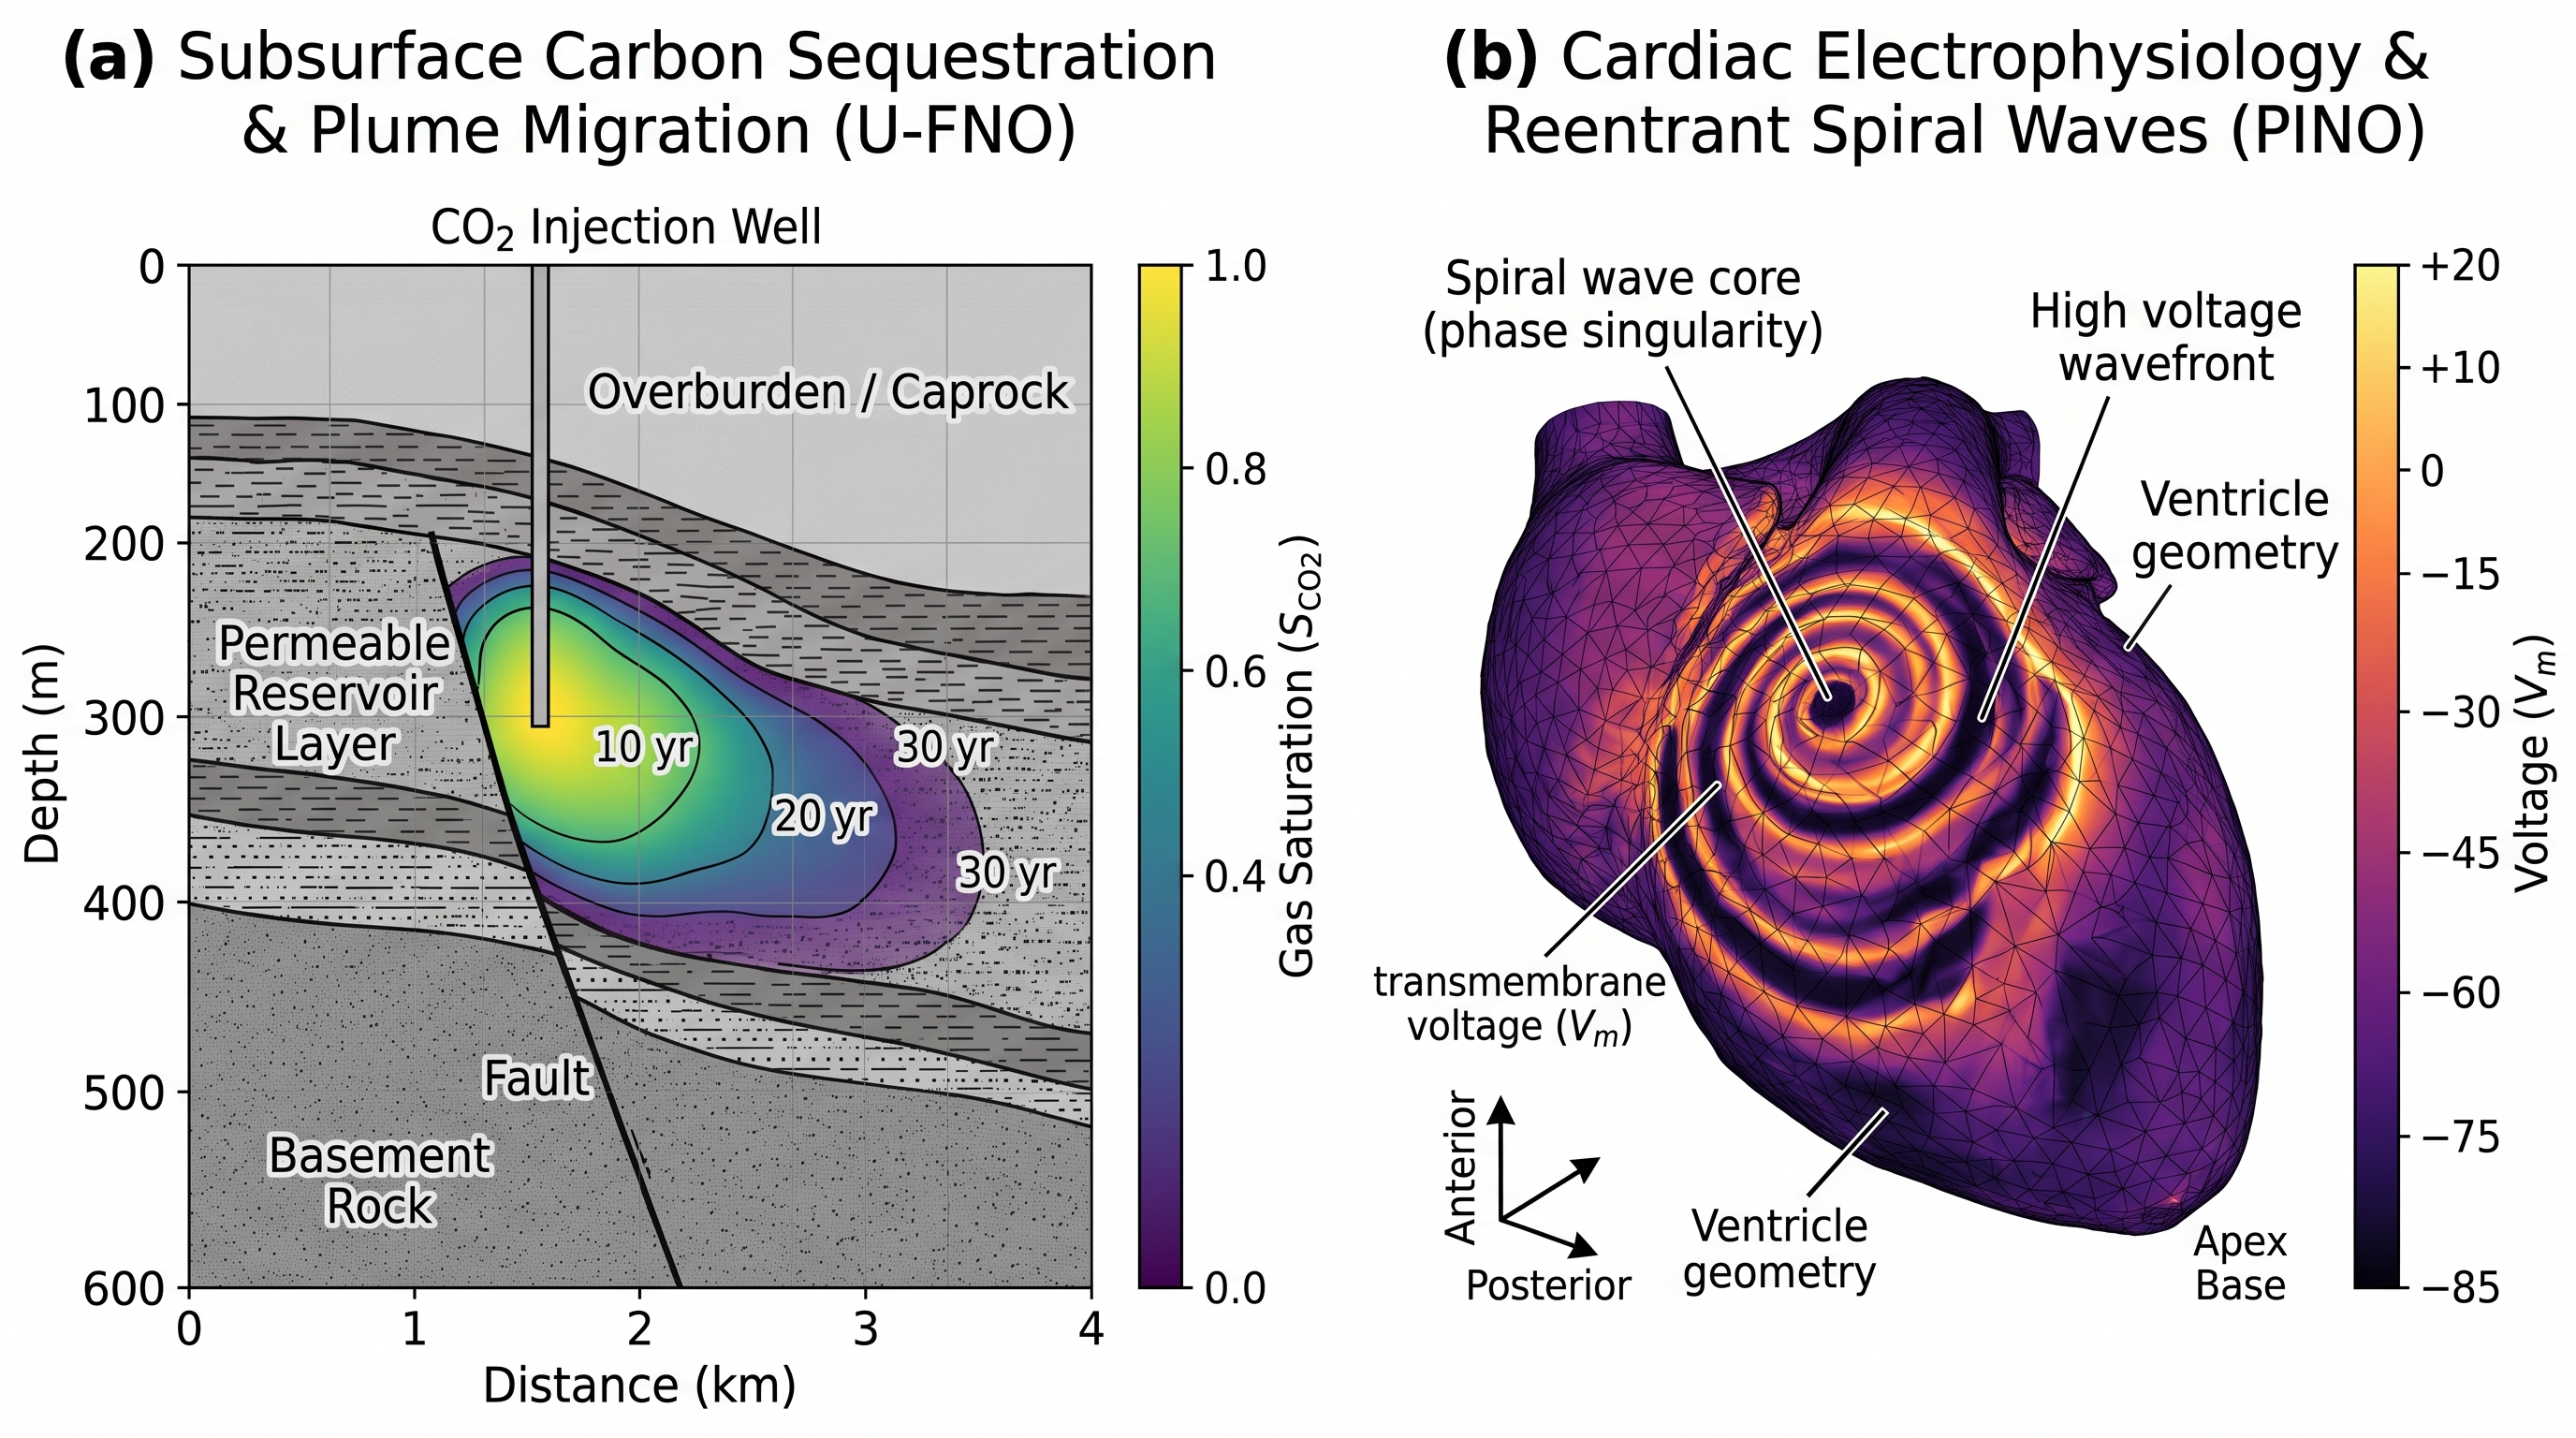
\includegraphics[width=0.80\textwidth]{fig_vol3_subsurface.jpg}
\caption{\textbf{Two-panel figure: subsurface $\mathrm{CO}_2$ plume migration
(panel~(a)) and cardiac reentrant spiral waves (panel~(b)).} Panel~(a), the
subject of this chapter, is a schematic cross-section of a saline-aquifer
$\mathrm{CO}_2$ storage site of the kind the U-FNO surrogate is trained to
simulate. Horizontal axis: distance, 0 to 4~km. Vertical axis: depth, 0 to
600~m, increasing downward. An impermeable overburden/caprock lies above
$\sim$110~m, a permeable reservoir layer between roughly 190 and 400~m, basement
rock below; a fault dips from 1.1~km at 200~m depth to the base of the section
near 2.2~km, and a vertical injection well enters at 1.6~km and terminates near
300~m. Filled contours give gas saturation $S_{\mathrm{CO}_2}$ on the scale 0 to
1; black contour lines mark the leading edge of the plume after 10, 20, and 30
years. Panel~(b), the subject of
\chapref{ch:part3-cardiac-electrophysiology-and-arrhythmia-d}, shows a reentrant
spiral wave of transmembrane voltage on a ventricle-shaped body rendered as a
triangular surface mesh, its colorbar labeled in millivolts from $-85$ to $+20$,
annotated at the spiral-wave core, the high-voltage wavefront, and the
anterior--posterior and apex--base axes; it is cited from
\chapref{ch:part3-cardiac-electrophysiology-and-arrhythmia-d} for that reading. Panel~(a) illustrates the physical
setting and the qualitative migration pattern; it is not a reproduction of a
figure from \cite{wen2022ufno}, whose benchmark is a two-dimensional radial
$(r,z)$ model without faulting, and no error figure quoted in this chapter is
read from either panel.}
\label{fig:vol3_sub}
\end{figure}
\index{plume migration!buoyant rise and lateral spreading}
\index{geological fault!as a leakage pathway}

% -----------------------------------------------------------------------------
\section{Performance vs. Classical Reservoir Solvers (Finite Difference)}
% -----------------------------------------------------------------------------

The baseline is not a straw solver. Commercial reservoir simulators of the class
used to generate the training data --- Eclipse, CMG, and the open-source research
toolkit MRST --- solve the coupled nonlinear system
\eqref{eq:ch34-cons-w}--\eqref{eq:ch34-cons-g} implicitly in time, with an
adaptive or fully implicit method (FIM) in which each step requires the residual
and its Jacobian and a Newton--Raphson iteration to convergence, upstream weighting
for the mobility, and a time-step controller that shortens steps whenever the
nonlinear solver struggles \cite{quarteroni2008numerical}. Wen et
al.~\cite{wen2022ufno} generated their data with the full-physics finite-difference
simulator Eclipse (e300) and report an average run time of about 10~min per
30-year case on one dedicated Intel Xeon E5-2670 core, each simulation using a
fully dedicated processor; the wider 10 to 30~min range per realization that this Part
carries forward is the working envelope for this class of problem. Against that, the trained U-FNO evaluates the same 30-year
evolution at 24 snapshots in 0.01 seconds on an NVIDIA A100 graphics processing
unit (GPU), for a reported 60,000$\times$ computational acceleration, with 1.6\%
gas saturation plume error and 0.68\% pressure error \cite{wen2022ufno}.
\index{fully implicit method (FIM)}
\index{reservoir simulator!Eclipse, CMG, MRST}

Those two percentages deserve to be read as what they are. In the study, 1.6\% is
the mean over 500 held-out cases of a mean absolute error computed \emph{inside the
separate-phase plume} --- the region where either the truth or the prediction is
nonzero --- and the accompanying standard deviation is about 1.1 percentage points;
0.68\% is the mean field relative error in pressure buildup, with a standard
deviation near 0.45. Neither number is a worst-case bound, and reporting the
plume error as ``below 1.6\%'' would misdescribe a distribution whose spread is
two-thirds of its center. The comparison against the plain FNO is more
informative still, because it shows what the U-Net path buys and what it costs. At
essentially the same parameter count, the plain FNO reaches a test plume error near
2.8\% and evaluates in about 0.005~s, while U-FNO reaches 1.6\% in 0.010~s: the
multi-scale path cuts the front error by roughly 40\% and doubles the inference
time, and the convolutional benchmark requires about three times the training data
to match the U-FNO's accuracy \cite{wen2022ufno}. The acceleration factor is
therefore not the largest available, and the architecture's claim is not speed but
speed at the accuracy where the physics concentrates.
\index{accuracy metrics!plume mean absolute error}
\index{speedup!as a property of the comparison setup}

Table~\ref{tab:ch34-cost} assembles the accounting, including the cost side that
an inference-time speedup invites the reader to forget. The speedup is a ratio of
two wall-clock numbers measured on specific hardware, and it moves when either
moves: the study itself notes that faster CPUs are available but would not
materially change the conclusion, which is true of the qualitative gap and false of
the factor --- a baseline twice as fast halves it. What does not depend on the
hardware is the shape of the cost curve. Simulation cost becomes a one-time
training cost plus a per-query cost four orders of magnitude or more below the
simulator's, and the data-generation cost is paid once and amortized across every
subsequent query. One qualification on the arithmetic: the $0.01$~s figure prices a
single network, and saturation and pressure are returned by two of them, so a query
that needs both fields costs about $0.02$~s and the honest ratio against a
$10$~min solve is nearer $3\times 10^{4}$ than $6\times 10^{4}$. The order of
magnitude is what the argument rests on, and it survives; the headline digit does
not.

\begin{table}[htbp]
\centering
\small
\caption{Cost and accuracy accounting for the U-FNO surrogate against the
finite-difference simulator that generated its training data, as reported by Wen et
al.~\cite{wen2022ufno} except that the 10--30~min run-time range is a figure this
Part carries without a primary reference. Simulator times are averages over 1,000 cases on one
dedicated Xeon core; surrogate times are averages over 500 held-out cases on one
A100 GPU, and the gas-saturation and pressure-buildup networks are evaluated
separately, so predicting both fields costs about twice the quoted 0.01~s.
Ensemble and training-set figures are arithmetic on the reported per-case costs,
not additional measurements.}
\label{tab:ch34-cost}
\begin{tabularx}{\textwidth}{l>{\raggedright\arraybackslash}X>{\raggedright\arraybackslash}X}
\toprule
 & \textbf{Implicit finite-difference simulator} & \textbf{U-FNO surrogate} \\
\midrule
Object computed &
  Cell-centered solution of \eqref{eq:ch34-cons-w}--\eqref{eq:ch34-cons-g}, every step &
  Approximate solution operator fitted on simulator output \\
Per-case wall clock &
  $\sim$10 min reported average; 10--30 min per realization in the inherited working range &
  0.010 s per output field, 24 snapshots \\
Ensemble of 1,000 cases &
  $\sim$170 core-hours &
  $\sim$10 s of GPU time \\
Accuracy, held-out cases &
  reference solution &
  1.6\% plume error ($\sigma \approx$ 1.1\%); 0.68\% pressure error ($\sigma \approx$ 0.45\%) \\
Data and training cost &
  none beyond the solve &
  5{,}500 simulator runs ($\approx$920 core-hours); 1{,}872 s per epoch \\
Held guarantees &
  local mass balance per control volume; entropy-satisfying fronts &
  fitted error statistics on the training distribution only \\
\bottomrule
\end{tabularx}
\end{table}

% -----------------------------------------------------------------------------
\section{Uncertainty, Conservation, and Failure Modes}
% -----------------------------------------------------------------------------

The consequence usually drawn from a $60{,}000\times$ factor --- that Monte Carlo
uncertainty quantification (UQ) sweeps over geological realizations become
practical --- is correct but needs the constraint attached to it. At
0.01~s per evaluation, an ensemble of $10^6$ realizations costs on the order of
$10^4$~s, a few hours on one GPU. What the surrogate does not do is make the
ensemble free: every member of the \emph{training} set still costs a simulator run,
and the reported study used 5{,}500 input--output mappings split 4{,}500 for
training and 500 each for validation and testing. The bottleneck therefore migrates
rather than disappears, from evaluation to data generation and to the question of
whether the sampling distribution covers the geology of interest. The permeability
fields are drawn from stationary variogram models of Gaussian, von K\'arm\'an, and
discontinuous facies type, generated with a geostatistical modeling package: the
same broad family of second-moment priors as the
log-permeability model \eqref{eq:ch25-darcy-measure} of
\chapref{ch:part2-canonical-pde-benchmarks-and-reference-wor}. The authors state
outright that they do not claim these maps model any real reservoir, and use them
to exercise the architecture across heterogeneous systems. A site whose
formation lies outside that family is therefore out of distribution, and the error
decomposition \eqref{eq:ch06-decomp} of \chapref{ch:part1-discretization-invariance-and-continuum-li}
--- statistical, truncation, and discretization error, in the three-way form
of \cite{subedi2024controlling} --- prices none of the misspecification of the
prior itself.
\index{uncertainty quantification (UQ)!Monte Carlo ensembles}
\index{out-of-distribution!geological transfer}
\index{permeability prior!variogram models}

The inverse problem is where the economics and the mathematics meet most
sharply. Estimating the permeability field from production and pressure data is a
Bayesian inverse problem \cite{stuart2010inverse}, and the Markov chain Monte Carlo
(MCMC) samplers that solve it need a forward evaluation at every proposal. A
surrogate fitted over the prior makes that affordable; one fitted only at a few
central permeability values does not, because the sampler will propose fields the
network has never seen and will answer them confidently. Here the distinction
between a fitted map and a solution operator stops being philosophical: the
posterior is computed against the surrogate's own validity domain, and a plausible
posterior concentrated on an unsupported region is worse than a divergent Newton
iteration, which at least announces itself.
\index{Bayesian inverse problem!permeability estimation}
\index{Markov chain Monte Carlo (MCMC)!surrogate evaluations}

Three specific failure modes deserve naming. The first is conservation. A finite
volume or finite difference discretization balances fluxes across each interface by
construction, so total injected mass is accounted for to solver tolerance; the
objective \eqref{eq:ch34-loss} controls an average relative error and implies no
such balance. Saturation bounds are the easy case --- $S_g \in [0,1]$ can be
imposed by an output transform, and $S_w = 1 - S_g$ by construction --- whereas
flux consistency is not, and putting the differential equation into the loss as in
\eqref{eq:pino_loss} penalizes the residual without restoring the local balance
identity. The second is the metric. \eqref{eq:ch34-rh} makes the front position the
carrier of the physics, and Part~I's analysis of \eqref{eq:ch09-gibbs} shows why an
aggregate relative $L^2$ number is forgiving of exactly the two errors that matter
here: an overshoot confined to a thin layer, and an interface displaced by a sub-grid
distance. The study also scores front location directly, as the maximum extent of
separate-phase $\mathrm{CO}_2$ above a saturation threshold of 0.01, and reports
relative error on that quantity --- 3.4\% for U-FNO against 9.2\% for the
convolutional benchmark \cite{wen2022ufno}. Front extent is what a
containment question is posed in, and no field average over the plume interior
substitutes for it.
\index{mass conservation!surrogate versus control-volume balance}
\index{L2@$L^2$ error!insensitivity to interface displacement}

The third is time. The network is trained on 24 snapshots of a 30-year injection
and returns the whole trajectory in one pass; it is not a time-stepper, and it
offers no mechanism for the centuries of post-injection migration on which
containment is actually judged. Extrapolating the learned operator beyond its
training horizon is the long-rollout problem of
Section~\ref{sec:ch09-rollouts}, where error growth compounds with each
self-conditioned step, and no reported figure in the multiphase literature supports
a century-scale claim. Resolution transfer is constrained in the same way from the
other side: adding the U-Net path to \eqref{eq:ch34-layer} costs the FNO its
discretization invariance, and the study is explicit that predictions at unseen
time steps are recovered only by resampling to the trained resolution, with a small
measured degradation in fit quality --- on a test set with the time step refined by
half, the reported $R^2$ for gas saturation falls from 0.993 to 0.987, while the
plain FNO, whose invariance is intact, moves from 0.989 to 0.986
\cite{wen2022ufno}. Geometry is constrained
likewise: the well is represented as a perforation of $0.1$~m radius, so any
quantity governed by the near-well gradient --- sandface pressure, injectivity,
skin --- is a property of the grid that produced it rather than of the continuum,
and a faulted three-dimensional multi-well field model is a different training
problem, not a larger version of this one. Architectures that
move the flexibility into the mesh, such as the geometry-informed operator
\cite{li2023geometry}, address that geometric limitation, but as
\chapref{ch:part1-open-theoretical-problems-and-mathematical} argues, adapting the
representation buys geometric reach and no additional regularity at the front.
\index{time extrapolation!beyond training horizon}
\index{discretization invariance!sacrificed by the U-Net path}
\index{wellbore!near-well resolution}

% -----------------------------------------------------------------------------
% Bridge to Chapter 3.5
% -----------------------------------------------------------------------------

The pattern established here transfers, with almost no modification, to the next
domain. A cardiac action potential is also a sharp traveling front: the Phase~0
depolarization upstroke is a transition of roughly a tenth of a volt across a
wavefront of order a millimeter wide, propagated through an anisotropic diffusion
tensor by a
reaction term that switches on abruptly, and its speed is likewise selected rather
than carried: in an excitable medium the front speed is set by the ratio of the
diffusivity to the excitability, not by smooth characteristics. The spectral obstruction of
\eqref{eq:ch09-jump-tail} and \eqref{eq:ch09-gibbs} applies to it with undiminished
force, the permeability tensor $\mathbf{K}(x)$ of \eqref{eq:ch34-flux} is replaced
by a fiber-orientation diffusion tensor with the same role of channeling the front
along preferred directions, and the multi-query driver reappears in patient
specificity rather than in geological uncertainty. What changes is the leverage the
equations themselves provide. In the subsurface, the simulator is the ground truth
and the residual form of the differential equation is at some distance from the
data; in cardiac
electrophysiology, the governing monodomain system is simple enough to write down,
cheap enough to evaluate a residual of, and uncertain enough in its parameters that
putting the differential equation into the objective becomes the operative
strategy. That is the subject of \chapref{ch:part3-cardiac-electrophysiology-and-arrhythmia-d}.

% -----------------------------------------------------------------------------
